\section{Cámaras y parámetros intrínsecos}

La forma en que los puntos tridimensionales del entorno se relacionan con los píxeles de una imagen tiene que ver con el modelo de cámara en cuestión. En las cámaras estenopeicas (también conocidas como cámaras \textit{pinhole}), modelamos la cámara como una caja donde una de sus paredes tiene un pequeño agujero, que interpretamos como un punto, por el que pasa la luz. La misma incide sobre la pared contraria, donde se ubica una grilla finita de puntos, dando lugar a la imagen. El proceso se conoce como transformación proyectiva.

\begin{figure}[H]
    \centering
    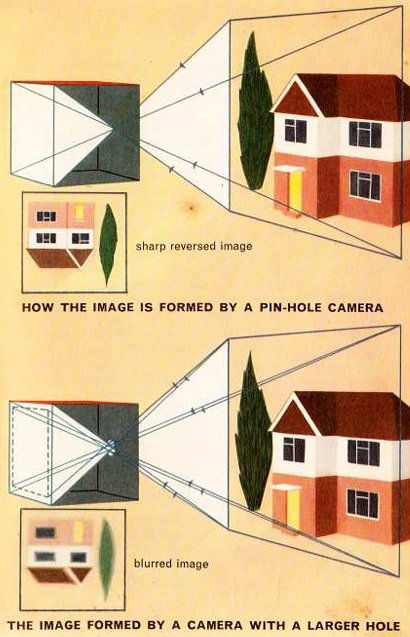
\includegraphics[width=0.5\linewidth]{../imagenes_marco_teorico/matriz_intrinseca.png}
    \caption{Efecto del tamaño del agujero en la proyección. En la parte inferior, la cámara posee un agujero más grande, obteniendo una imagen más borrosa al dejar pasar más luz. Imagen extraida de \cite{howcameraworks}}
    \label{fig:matriz_intrinseca}
\end{figure}

Al pasar por el agujero, la luz se proyecta invertida sobre el plano. Como se observa en la Figura \ref{fig:matriz_intrinseca}, esto sucede al pasar por el agujero, cuya forma, junto a la de la cámara, afectan la imagen resultante. En el modelo, se asume que el agujero es infinitesimalmente pequeño, pero en la práctica eso es físicamente imposible. Por lo tanto, se utilizan lentes que permiten obtener imágenes nítidas al asemejarse al ideal, fijando un punto a través del cual se proyecta la luz, conocido como foco.

Para controlar la diferencia entre el modelo y la realidad, es necesario conocer la geometría de la cámara. En especial, la distancia focal, que es la distancia entre la lente y el foco; y el punto principal, que es la ubicación del píxel de la imagen donde se intersecta el rayo óptico, es decir, el punto donde el centro de la lente se proyecta sobre el plano imagen. En la Figura \ref{fig:lente_grafico11} se muestra una representación de estos parámetros, que resultan fundamentales para modelar la proyección de los puntos sobre la imagen.

\begin{figure}[H]
    \centering
    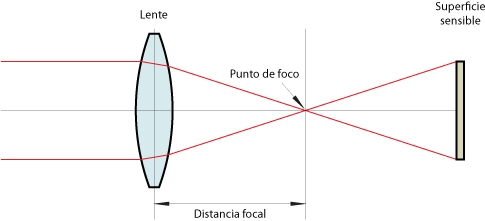
\includegraphics[width=0.5\linewidth]{../imagenes_marco_teorico/lente_grafico11.png}
    \caption{Representación de los parámetros intrínsecos. La superficie sensible es la que recibe la luz para formar la imagen. La línea perpendicular a ella que pasa por el foco es donde se encuentra el punto principal. Imagen extraida de \cite{bokebinario}}
    \label{fig:lente_grafico11}
\end{figure}

Estos parámetros se agrupan en la llamada matriz intrínseca de la cámara, que describe la transformación entre coordenadas del plano de la imagen y coordenadas de píxel del siguiente modo:

\begin{equation}
\mathbf{K} =
\begin{pmatrix}
f_x & 0   & c_x \\
0   & f_y & c_y \\
0   & 0   & 1
\end{pmatrix}
\end{equation}

con $f_x, f_y$ focales en píxeles, y $c_x, c_y$ posición del punto principal. Los valores se pueden obtener a partir de la información del fabricante de la cámara, o mediante un procedimiento de calibración, formalizado en la literatura por Zhang et al. \cite{calibracion_camara}.